\documentclass{article}
\usepackage[utf8]{inputenc}
\usepackage{natbib}
\usepackage{amsmath}

\title{Replicate : A Hybrid System Model of Seasonal Snowpack Water Balance}
\author{Fred Eisele }
\date{2014 December 1}

\usepackage[showframe=true]{geometry}
\geometry{verbose, tmargin=0pt, bmargin=90pt, lmargin=90pt, rmargin=90pt}

\begin{document}

\maketitle

\section{Motivation for Work}

Systems with long time steps may be modeled with hybrid automata
\citep{kerkez2010swb}.
This project replicates part of the work involved with modeling
the seasonal snowpack water balance and the snow-water-equivalence (SWE).
The SWE is important in estimations of the water available
for consumption in the winter snowpack.
This is of particular importance in the desert west of the USA.
As policies are developed concerning water rights it
will be useful to have accurate models and simulations.

\section{Physical Model}

The problem space primarily concerns the Spring thaw.
We can assume that there is no additional snowfall,
no appreciable sublimation and that there is no
heat transfer by convection to the atmosphere.
The conversion of the snowpack to run-off is due solely
to radiative effects, insolation, heating from the sun,
and night time cooling.

\subsection{Diurnal Insolation}

In the paper the insolation was obtained emperically.
For my purpose the solar intensity is modeled as a sine
function during the day and clipped for night.
Typical daily insolation values are about $3 \text{kW-hr/day}$.

\begin{align}
u(t)_{solar} &= a \sin{2 \pi t} \\
\int_0^{1 day} u(t)_{solar} dt &= \frac{a}{2 \pi} \\
  &\approx 3 \text{kW-hr/day} \\
a &\approx 30,000 kJ/day
\end{align}

This is coupled with a constant cooling to produce heating function.
\begin{align}
u(t)_{space} &\approx 0.1 \text{kW/$m^2$} \\
   &\approx 8600 \text{kJ/$m^2$-day} \\
u(t) &= 30,000 \sin{2 \pi t} - 8600 \text{kJ/$m^2$-day}
\end{align}


\subsection{Capacitive Heating}

The heat capacity of snow is the same as that of ice.

\begin{align}
\frac{dT}{dt} &= \frac{u(t)}{M_{snow} C_{snow}}
\end{align}
This is used only in the Frozen mode as that is
the only mode where the temperature changes.

\subsection{Melting}

The latent heat of fusion for snow is the same as for ice.
\begin{align}
\frac{dM_{water}}{dt} &= -\frac{dM_{ice}}{dt} \\
  &= \frac{u(t)}{L_f}
\end{align}
This is not used in the Frozen mode as there is no water present.

\subsection{Compaction}

Snow is a mixture of ice and air.
The specific composition is varied and several models exist.
The compaction behavior over time is complex but can
be well described by formula.
Starting with the half-saturation formula where $A$ ($kg/m^2$) is the
maximum saturation level and $B$ ($days$) is the
half-saturation time.
Taking the derivative gives the compaction rate.

\begin{align}
\rho_{snow}(t) &= \frac{A}{1 + B/t} \\
\frac{d\rho_{snow}(t)}{dt} &= \frac{A B}{(B + t)^2} \\
\end{align}

Computing the time when a particular density is reached and
substituting gives a function for the compaction rate
as a function of density.

\begin{align}
t &= \frac{\rho_{snow} B}{A - \rho_{snow}} \\
\frac{d\rho_{snow}(t)}{dt}
    &= \frac{A}{B (1 + \frac{\rho_{snow}(t)}{A - \rho_{snow}(t)}) }
\end{align}

Compaction occurs in all modes except in the
absence of a snowpack.


\subsection{Adsorbtion}

Snow acts as a sponge, adsorbing water into its matrix.
This fact distinguishes the thawing and melting modes.
The thawing mode is characterized by the snow's ability
to adsorb more water, while the melting mode is supersaturated
and additional conversion of ice into water results in run-off.
This idea is expressed in the volumetric water content of the snow,
$\theta_{snow}$.

\begin{align}
\theta_{snow} &= \frac{V_{water}}{V_{total}} \\
   &= \frac{M_{water}/ \rho_{water}}{M_{snow}/\rho_{snow}}
\end{align}

The maximum $\theta_{snow}$ signals the transition between
modes, designated $\theta_{r}$.
The mass of water in the saturated snowpack follows directly.
And, differentiating by parts once gives the rate that the water in the
snowpack is changing.

\begin{align}
M_{water}  &= \theta_{r} \rho_{water}
      \frac{M_{ice}}{\rho_{snow} - \theta_{r} \rho_{water}} \\
\frac{d M_{water}}{dt} &=  \theta_{r} \rho_{water}
   \left[ \frac{\frac{d M_{water}}{dt} (\rho_{snow} - \theta_{r} \rho_{water})
                  - M_{ice} \frac{d \rho_{snow}}{dt} }
          {(\rho_{snow} - \theta_{r} \rho_{water})^2} \right]
\end{align}

Intuitively this relation makes sense.
A higher density in the snowpack results is a lower adsorbtivity.
These provide a sufficient physical model to construct the hybrid model.


\section{Hybrid Model}

The hybrid model is a bulk model for an arbitrary core
sample of the snowpack.
It has two top level modes, one representing the absence
of snow, and the other representing the presence of a snowpack.
The snowpack mode is further discriminated into three modes:
frozen, thawing and melting.

\begin{figure}
\centering
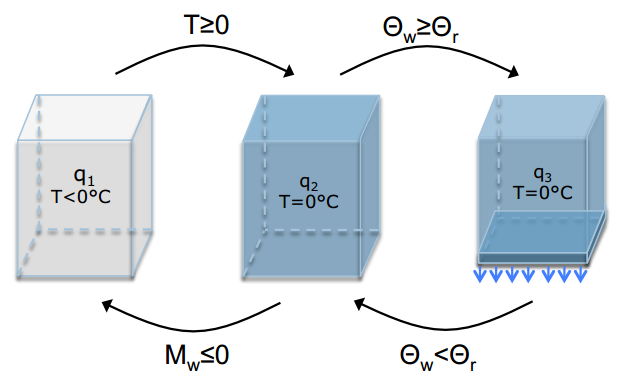
\includegraphics{discrete_modes.png}
\caption{The snowpack modes}
\label{fig:snowpack_modes}
\end{figure}

\subsection{Discrete Model}

\subsection{No Snowpack}

\subsection{Frozen : Sub-Zero}

\subsection{Thawing : Unsaturated}

\subsection{Melting : Saturated}

\section{Work Performed}

I have a hybrid model based on the recommended
Stateflow\textregistered Simulink\textregistered
design patterns \citep{matlab2009ssdp}.
I am using discrete time steps (rather than continuous) as the
physical system has a large degree of variability.

\section{Modeling Issues}

Starting with a continuous model reveiled semantic
issues with embedding a continuous integrator in a SimuLink function.
Switching to a discrete integrator resolved these issues but
there are still questions related to how to appropriately
model the differential equations.

The other significant issue is the proper calibration of the model.
Typically the models produced with
Stateflow\textregistered Simulink\textregistered are working
with time frames in the one second region.
This problem uses time frames in the hour or day region.

A minor issue is that the paper does not describe
the input in much detail.
The data they use is that recorded in various surveys.
This will be approximated in my model with a sine wave
that immitates the diurnal insolation with the trough
giving up energy.


\section{Physical Constants and Conditions}

\begin{align}
u(t) &= a \sin{2 \pi t} - c_{rad} \\
 &= - c_{rad} \\
U(t) &= \frac{a \cos{2 \pi t}}{2 \pi} |_0^{1/2} - c_{rad} t |_0^1 \\
  &= 3 \text{ kW-hr/$m^2$ } \\
  &= 10,800 \text{ kJ/$m^2$ } \\
c_{rad} &= 800 \text{ kJ/$m^2$-day } \\
a &= (10,800 - c_{rad}) \times 2 \pi \text{ kJ/$m^2$-day } \\
 &= 20,000 \pi \text{ kJ/$m^2$-day } \\
 &\approx 63,000 \text{ kJ/$m^2$-day }
\end{align}

Where $t$ is measured in days.
$A$ is the average daily insolation.
A reasonable, Springtime, value for $A$ is near $3 \text{kW-hr}/m^2$.

\begin{align}
 C_{ice} &= 2.05 \text{ kJ/kg-K} \\
 C_s &= C_{ice} \\
\theta_r &= 0.01 \\
L_f &= 334 \text{ kJ/kg} \\
\rho_w &= 1000 \text{ kg/$m^3$} \\
A &= 450 \text{ kg/$m^3$} \\
B &= 20 \text{ days}
\end{align}

 \section{Conclusion}

\bibliographystyle{plain}
\bibliography{references}

\end{document}
